\documentclass[12pt, twoside]{article}
\usepackage[letterpaper, margin=1in, head=30pt, headsep=0.1in]{geometry}
\usepackage[english]{babel}
\usepackage[utf8]{inputenc}
\usepackage{amsmath}
\usepackage{amsfonts}
\usepackage{amssymb}
\usepackage{tikz}
%\usetikzlibrary{quotes, angles}

\usepackage{graphicx}
\usepackage{enumitem}
\usepackage{multicol}

%\usepackage{pgfplots}
%\pgfplotsset{width=10cm,compat=1.9}
%\usepgfplotslibrary{statistics}
%\usepackage{pgfplotstable}
%\usepackage{tkz-fct}
%\usepackage{venndiagram}

\usepackage{fancyhdr}
\pagestyle{fancy}
\fancyhf{}
\renewcommand{\headrulewidth}{0pt} % disable the underline of the header
\raggedbottom
\newif\ifmeta
\metatrue %print standards and topics tags

\title{Math AI Worksheet Generator and Formative Assessment System}
\author{Chris Huson}
\date{August 2019}

\fancyhead[RE]{\thepage}
\fancyhead[RO]{\thepage \\ Name: \hspace{3cm}}
%\fancyhead[L]{BECA / Dr. Huson / 10th Grade Geometry\\* 7 June 2019}
%
%\begin{document}
%\subsubsection*{13.7 Homework: Cross sections, distance applications}
\fancyhead[L]{BECA / Dr. Huson / Geometry 02-Midpoint+distance\\* pset ID: 23}

\begin{document}

\subsubsection*{2-5HW-Perimeter.tex}
\begin{enumerate}
\item Given the rectangle $ABCD$ shown below, with $AB=11$ and $BC=2.5$. Find the perimeter of the rectangle.
    \begin{flushleft}
    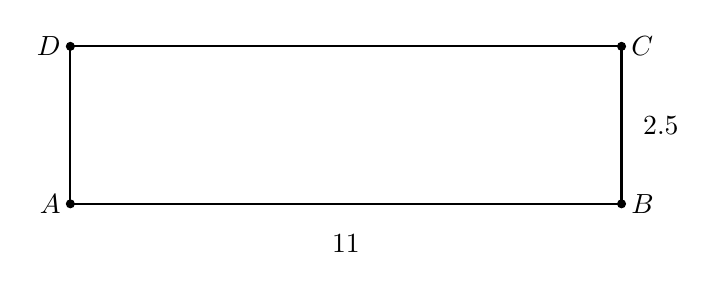
\begin{tikzpicture}
      \draw [-, thick] (0,0)--(7,0)--(7,2)--(0,2)--cycle;
      \draw [fill] (0,0) circle [radius=0.05] node[left]{$A$};
      \draw [fill] (7,0) circle [radius=0.05] node[right]{$B$};
      \draw [fill] (7,2) circle [radius=0.05] node[right]{$C$};
      \draw [fill] (0,2) circle [radius=0.05] node[left]{$D$};
      \node at (7.5, 1){2.5};
      \node at (3.5, -0.5){11};
    \end{tikzpicture}
    \end{flushleft} \vspace{2cm}  

\item Given $\overleftrightarrow{PQ}$ as shown on the number line, with $P=-3.25$ and $Q=4.5$. \\[20pt] % Midpoint
    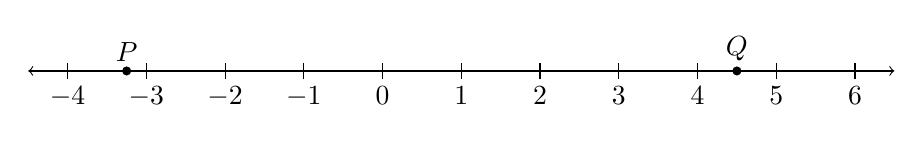
\begin{tikzpicture}
      \draw [<->] (-4.5,0)--(6.5,0);
      \foreach \x in {-4,...,6} %2 leading for diff!=1
        \draw[shift={(\x,0)},color=black] (0pt,-3pt) -- (0pt,3pt) node[below=5pt]  {$\x$};
        \draw [fill] (-3.25,0) circle [radius=0.05] node[above] {$P$};
        \draw [fill] (4.5,0) circle [radius=0.05] node[above] {$Q$};
    \end{tikzpicture} \\ \bigskip
    What is the exact distance on the number line between the points $P$ and $Q$? \vspace{3cm}  

\item Given two complementary angles, $\angle A$ and $\angle B$, with $m\angle A = 43^\circ$. Find the measure of $\angle B$. \vspace{2.5cm} 

\item Angles $P$ and $Q$ are supplementary. $m\angle P = 23^\circ$. Find $m\angle Q$.
    
    \newpage

\item Given $\overline{ABC}$, $AB=27$, and $AC=161$.\\ [0.5cm]
    Find ${BC}$.\\[1.5cm]
        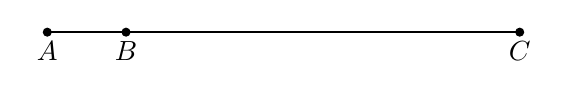
\begin{tikzpicture}
          \draw [-, thick] (1,0)--(7,0);
          \draw [fill] (1,0) circle [radius=0.05] node[below]{$A$};
          \draw [fill] (2,0) circle [radius=0.05] node[below]{$B$};
          \draw [fill] (7,0) circle [radius=0.05] node[below]{$C$};
        \end{tikzpicture}\\[1.5cm]
        The postulate used in this problem is the \rule{6cm}{0.15mm}.
        \vspace{1.5cm}

\item Given the diagram shown below. \vspace{0.25cm}
    \begin{enumerate}
      \item  Measure the angle $BED$. $m \angle BED = $ \rule{4cm}{0.15mm} \bigskip
      \item Name an angle that is supplementary to $\angle AEB$: \rule{4cm}{0.15mm} \bigskip
      \item Name an angle that is complementary to $\angle BEC$: \rule{4cm}{0.15mm}
    \end{enumerate}
    \vspace{1cm}
    \begin{center}
    \begin{tikzpicture}[scale=1.5]
      \draw [->, thick] (0,0)--(125:5);
      \draw [<->, thick] (-5,0)--(5,0);
      \draw [->, thick] (0,0)--(0,4);
      \draw (0,0)++(0.3,0)--++(0,0.3)--+(-0.3,0);
      %\draw [fill] (-1,2.5) circle [radius=0.05] node[left ]{$B$};
      \draw [fill] (125:3) circle [radius=0.05] node[below left]{$B$};
      \draw [fill] (-4,0) circle [radius=0.05] node[below]{$A$};
      \draw [fill] (0,0) circle [radius=0.05] node[below]{$E$};
      \draw [fill] (0,3) circle [radius=0.05] node[left]{$C$};
      \draw [fill] (4,0) circle [radius=0.05] node[below]{$D$};
    \end{tikzpicture}
    \end{center}


\end{enumerate}
\end{document}